
\subsection{DLC24}
\label{sec:baseline-vs-KB6:dlc24}

\begin{figure}[!ht]
\begin{center}
	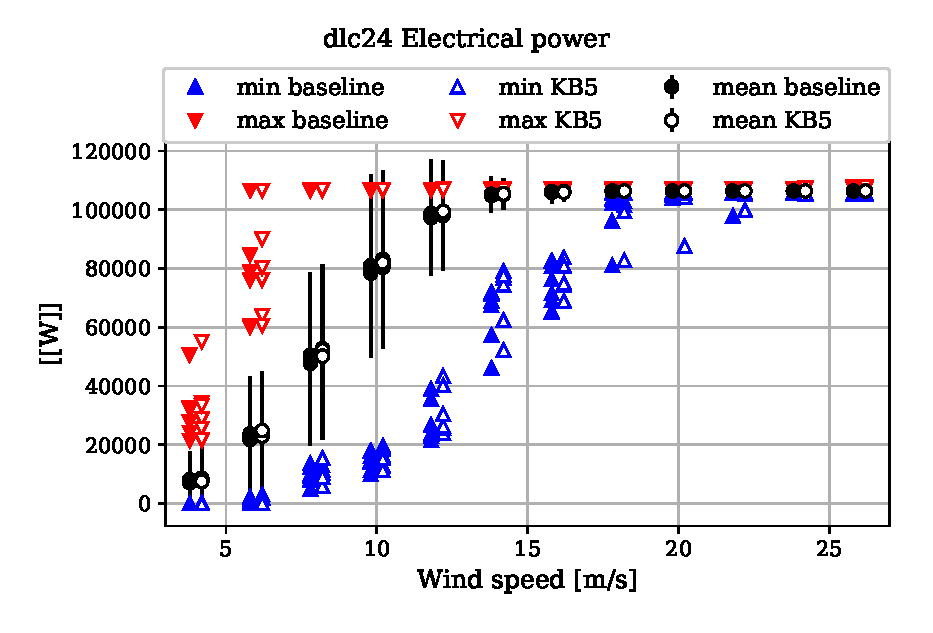
\includegraphics[width=.85\linewidth]{figures/baseline-vs-KB6/dlc24/DLL-generator_servo-inpvec-2_AA0007_AA0003.eps}
\end{center}
\caption{Electrical power [W], excluding losses.}
\label{fig:baseline-vs-KB6:dlc24:power}
\end{figure}

\begin{figure}[!ht]
\begin{center}
	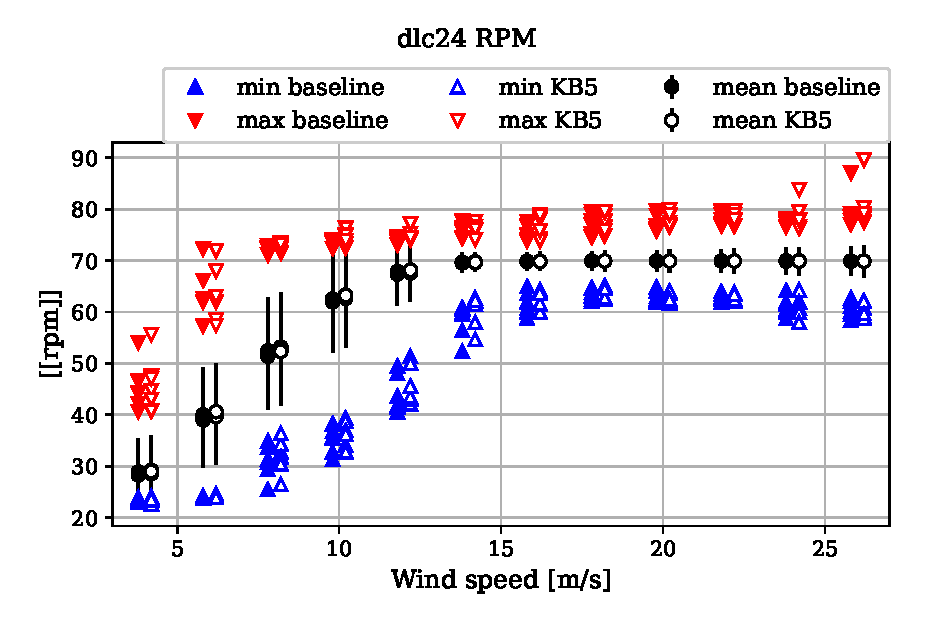
\includegraphics[width=.85\linewidth]{figures/baseline-vs-KB6/dlc24/bearing-shaft_rot-angle_speed-rpm_AA0007_AA0003.eps}
\end{center}
\caption{Rotor speed [RPM]}
\label{fig:baseline-vs-KB6:dlc24:rpm}
\end{figure}

\begin{figure}[!ht]
\begin{center}
	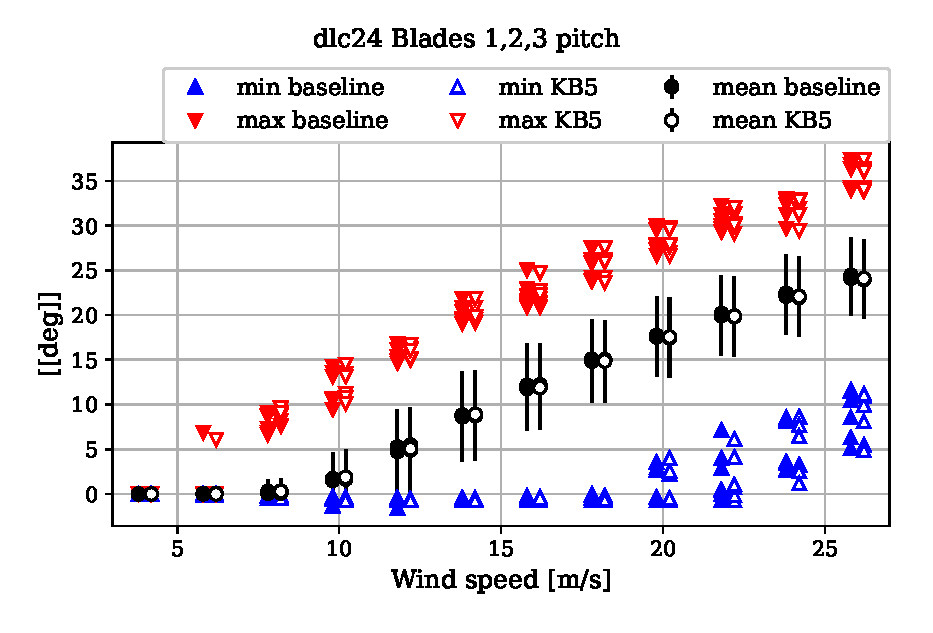
\includegraphics[width=.85\linewidth]{figures/baseline-vs-KB6/dlc24/bearing-pitch1-angle-deg_AA0007_AA0003.eps}
\end{center}
\caption{Blade 1, 2 and 3 pitch angles [deg]}
\label{fig:baseline-vs-KB6:dlc24:pitch}
\end{figure}

\begin{figure}[!ht]
\begin{center}
	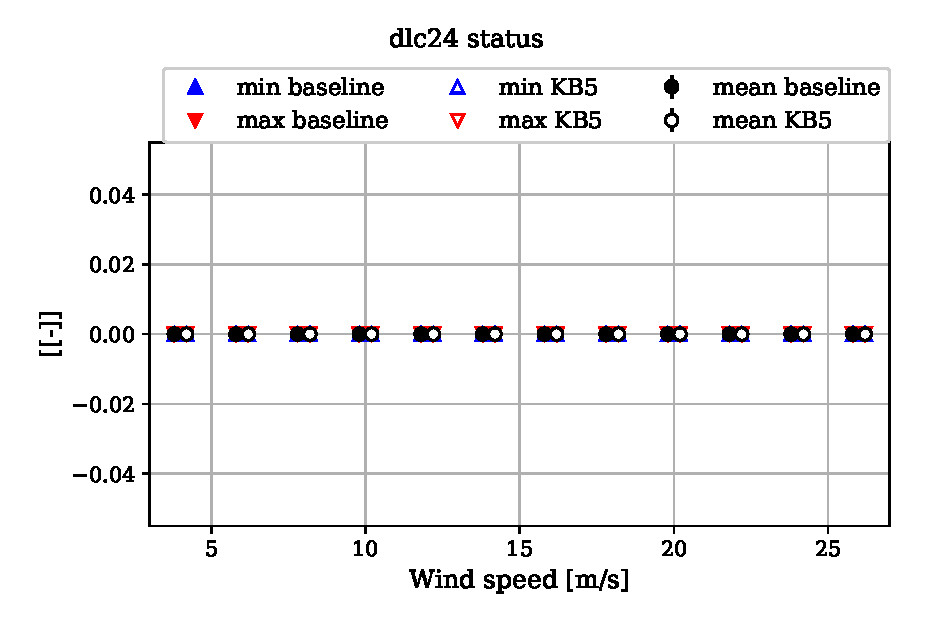
\includegraphics[width=.85\linewidth]{figures/baseline-vs-KB6/dlc24/DLL-dtu_we_controller-inpvec-22_AA0007_AA0003.eps}
\end{center}
\caption{Controller status flag [0-6], 0: normal operation, 1: shut down due to overspeed}
\label{fig:baseline-vs-KB6:dlc24:status}
\end{figure}

\begin{figure}[!ht]
\begin{center}
	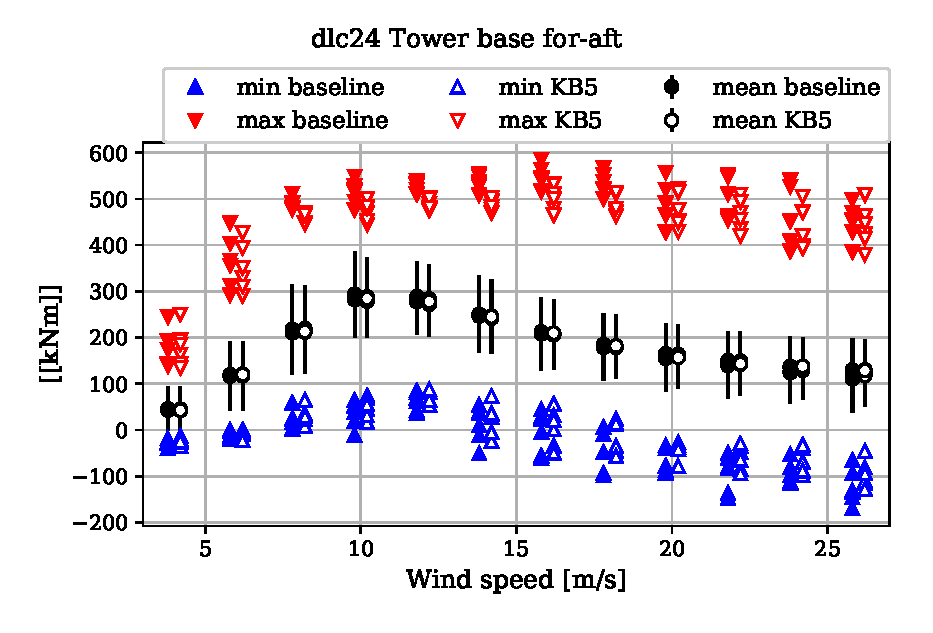
\includegraphics[width=.85\linewidth]{figures/baseline-vs-KB6/dlc24/tower-tower-node-001-momentvec-x_AA0007_AA0003.eps}
\end{center}
\caption{Tower base for-aft bending moment [kNm]}
\label{fig:baseline-vs-KB6:dlc24:tower-base-fa}
\end{figure}

\begin{figure}[!ht]
\begin{center}
	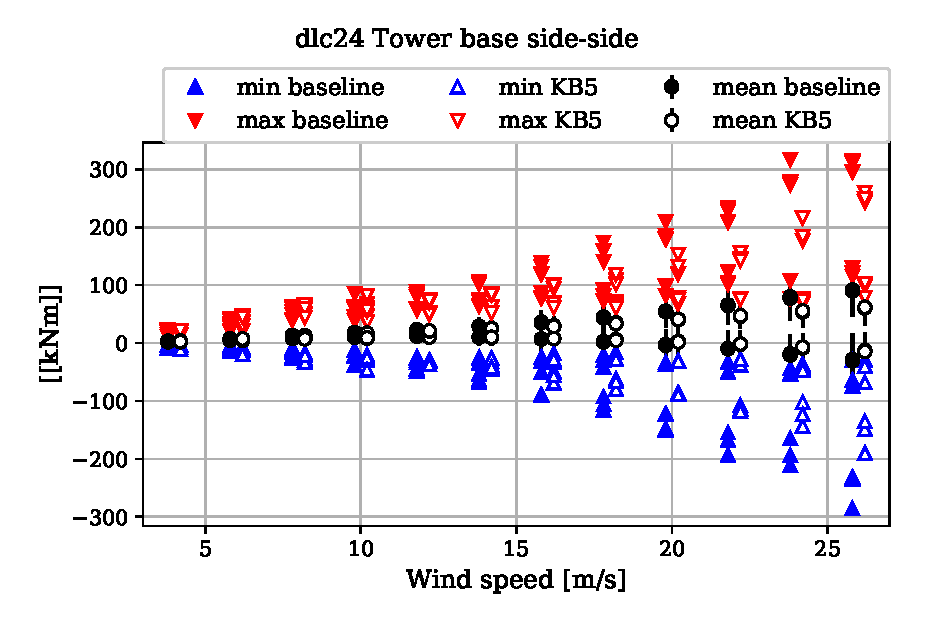
\includegraphics[width=.85\linewidth]{figures/baseline-vs-KB6/dlc24/tower-tower-node-001-momentvec-y_AA0007_AA0003.eps}
\end{center}
\caption{Tower base side-side bending moment [kNm]}
\label{fig:baseline-vs-KB6:dlc24:tower-base-ss}
\end{figure}

\begin{figure}[!ht]
\begin{center}
	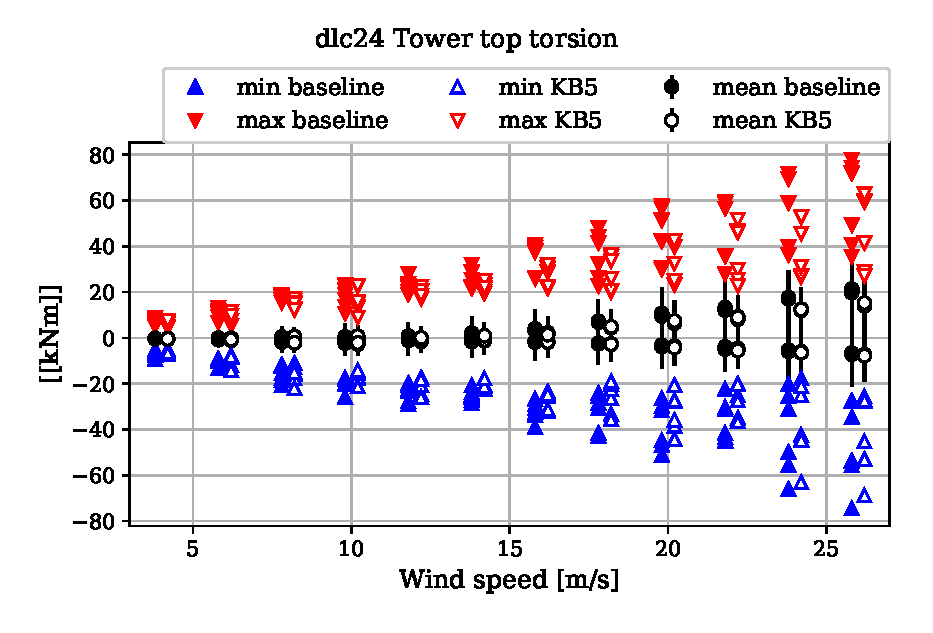
\includegraphics[width=.85\linewidth]{figures/baseline-vs-KB6/dlc24/tower-tower-node-004-momentvec-z_AA0007_AA0003.eps}
\end{center}
\caption{Yawing moment tower top [kNm]}
\label{fig:baseline-vs-KB6:dlc24:tower-top-yaw}
\end{figure}

\begin{figure}[!ht]
\begin{center}
	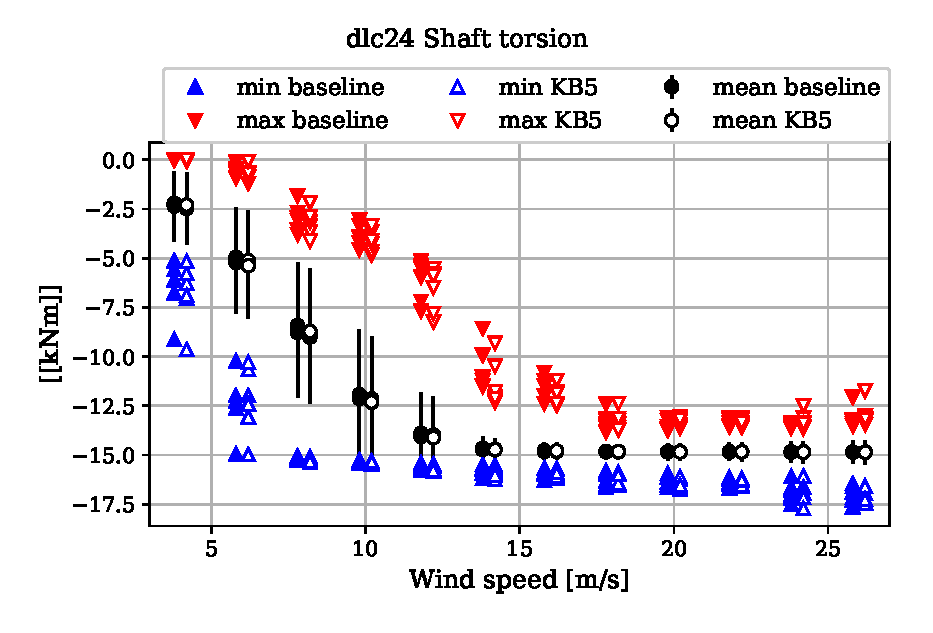
\includegraphics[width=.85\linewidth]{figures/baseline-vs-KB6/dlc24/shaft-shaft-node-001-momentvec-z_AA0007_AA0003.eps}
\end{center}
\caption{Shaft torsion moment [kNm]}
\label{fig:baseline-vs-KB6:dlc24:shaft-torsion}
\end{figure}

\begin{figure}[!ht]
\begin{center}
	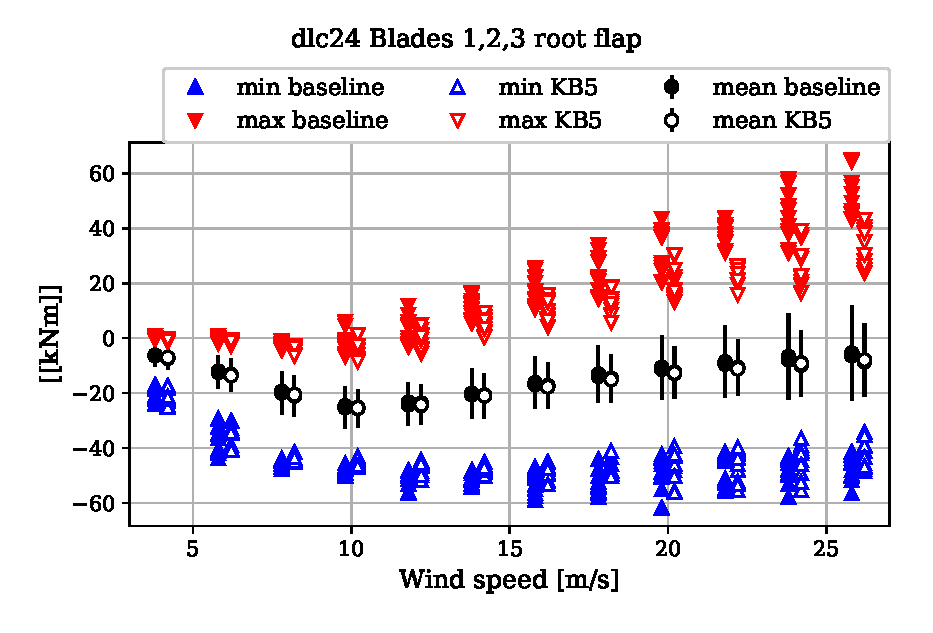
\includegraphics[width=.85\linewidth]{figures/baseline-vs-KB6/dlc24/blade1-blade1-node-001-momentvec-x_AA0007_AA0003.eps}
\end{center}
\caption{Blade root 1, 2 and 3 flap-wise bending moments [kNm] (pitching coordinates)}
\label{fig:baseline-vs-KB6:dlc24:blade-root-flap}
\end{figure}

\begin{figure}[!ht]
\begin{center}
	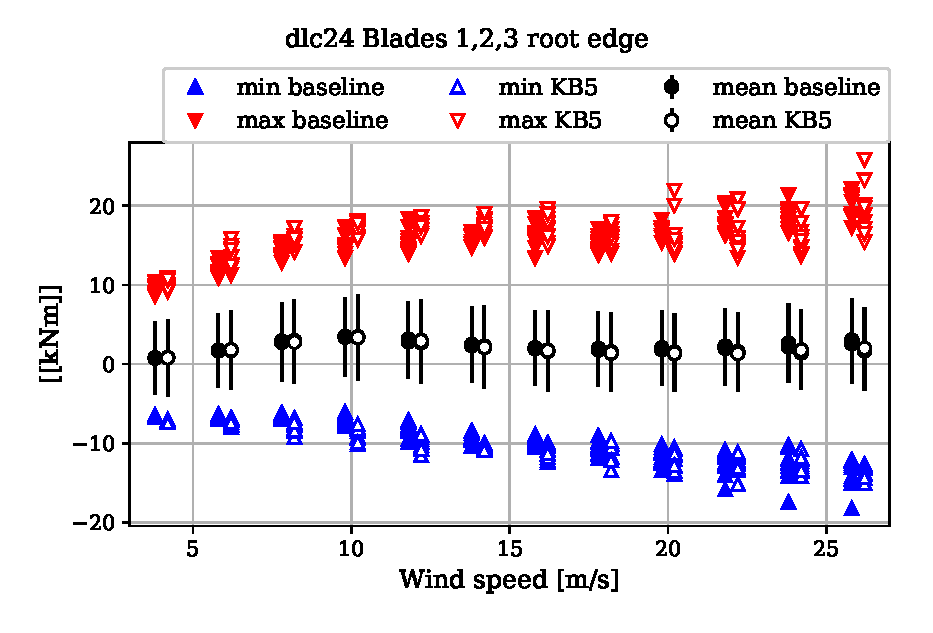
\includegraphics[width=.85\linewidth]{figures/baseline-vs-KB6/dlc24/blade1-blade1-node-001-momentvec-y_AA0007_AA0003.eps}
\end{center}
\caption{Blade root 1, 2 and 3 edge-wise bending moments [kNm] (pitching coordinates)}
\label{fig:baseline-vs-KB6:dlc24:blade-root-edge}
\end{figure}

\begin{figure}[!ht]
\begin{center}
	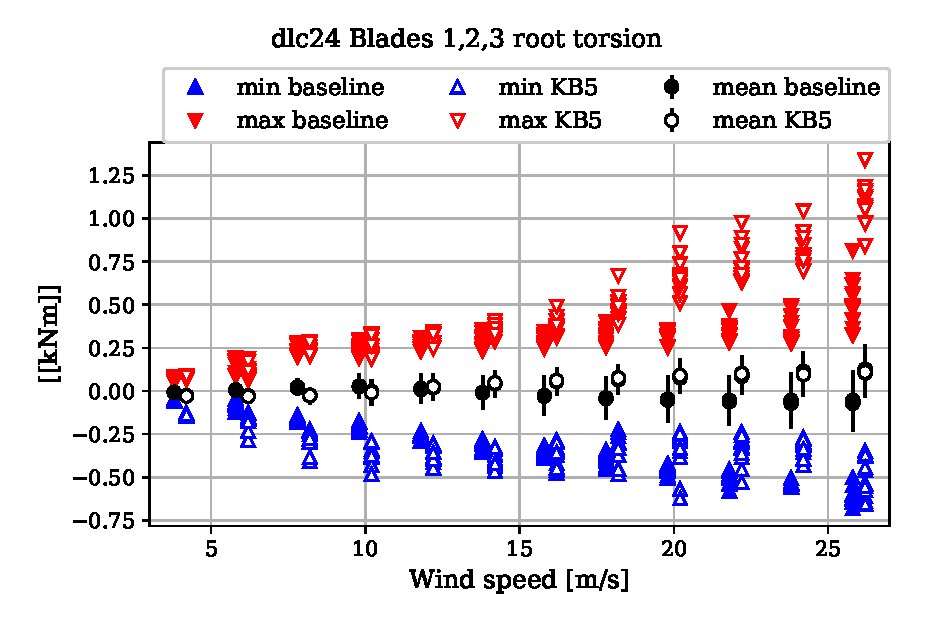
\includegraphics[width=.85\linewidth]{figures/baseline-vs-KB6/dlc24/blade1-blade1-node-001-momentvec-z_AA0007_AA0003.eps}
\end{center}
\caption{Blade root 1, 2 and 3 torsion bending moments [kNm] (pitching coordinates)}
\label{fig:baseline-vs-KB6:dlc24:blade-root-torsion}
\end{figure}

\begin{figure}[!ht]
\begin{center}
	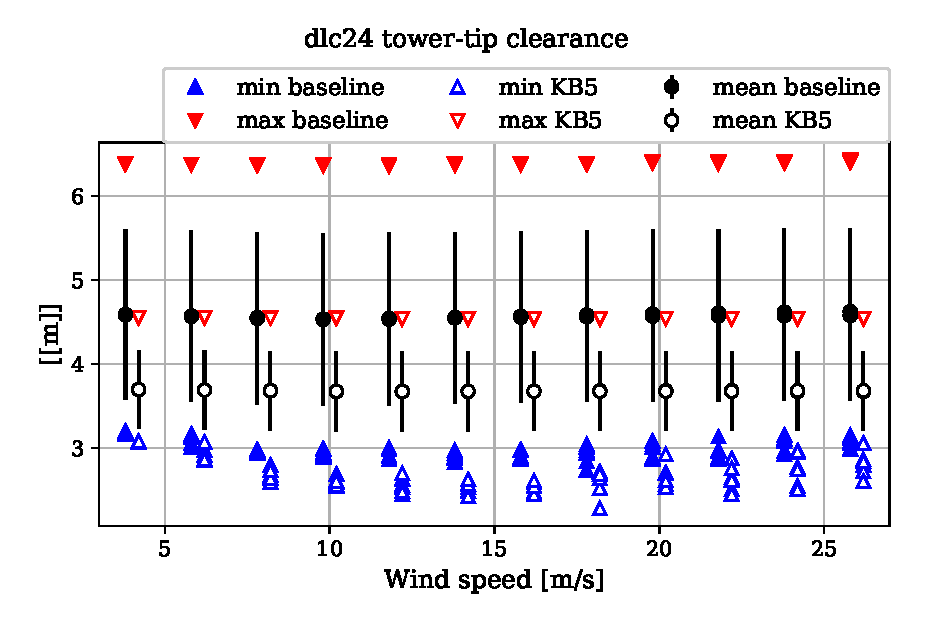
\includegraphics[width=.85\linewidth]{figures/baseline-vs-KB6/dlc24/DLL-towerclearance_mblade-inpvec-1_AA0007_AA0003.eps}
\end{center}
\caption{Minimum tower to blade tip distance [m] (consider only the minima)}
\label{fig:baseline-vs-KB6:dlc24:tower-tip-clearance}
\end{figure}

